\documentclass[tikz,border=2pt]{standalone}
\usepackage{tikz}
\usepackage{amsmath,amssymb,amsthm}
\usetikzlibrary{arrows,arrows.meta,positioning,shapes,calc}

% Custom macros used in the textbook
\newcommand{\R}{\mathbb{R}}
\newcommand{\N}{\mathbb{N}}
\newcommand{\Z}{\mathbb{Z}}
\newcommand{\C}{\mathbb{C}}

\begin{document}
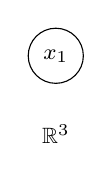
\begin{tikzpicture}[
    neuron/.style={circle, draw, minimum size=0.7cm, font=\footnotesize},
    arrow/.style={->, >=stealth}
]
\node[neuron] (x1) at (0, 0) {$x_1$};
\node[font=\footnotesize] at (0, -1) {$\R^3$};
\end{tikzpicture}
\end{document}
